%% Short data paper template
%% Created by Simon Hengchen and Nilo Pedrazzini for the Journal of Open Humanities Data (https://openhumanitiesdata.metajnl.com)

\documentclass{article}
\usepackage[english]{babel}
\usepackage[utf8]{inputenc}
\usepackage{johd}
\usepackage{amsthm}
\usepackage{amsmath}

% Definir un nuevo estilo de teorema sin cursiva
\newtheoremstyle{customdef} % Nombre del estilo
  {}    % Espaciado arriba
  {}    % Espaciado abajo
  {\normalfont} % Cuerpo del texto en fuente normal (sin cursiva)
  {}    % Indentación
  {\bfseries} % Título en negrita
  {}   % Puntuación después del título
  { }   % Espaciado después del título
  {\thmname{#1}\thmnote{ \textbf{#3}}} % Formato del título

% Aplicar el nuevo estilo
\theoremstyle{customdef}
\newtheorem{definition}{Definition}
\newtheorem{lemma}{Lemma}

\title{EVE Astar: A system-pathfinder solver}

\author{Javier Martín Pizarro\\
        \small Independent, Universidad Carlos III de Madrid, Madrid, Spain \\}

\begin{document}
\maketitle

\begin{abstract} 
\noindent This paper aims to analyze and replicate the pathfinding algorithm used in EVE Online for navigating between star systems. It explores the underlying algorithm, the heuristics applied, and their impact on route optimization. Additionally, the paper discusses the advantages and limitations of this approach in the context of in-game travel. \end{abstract}

\noindent\keywords{A* algorithm, pathfinding, heuristics}\\

\section{Overview}
\paragraph{Context} EVE Online is considered one of the biggest spatial MMORPG, with more than 7500 systems to travel to. All those systems are connected between each other, conforming a graph $G(V,E)$. Players can travel through different systems following a determined path that can be calculated using an internal tool - a pathfinding solver.

This solver has several use cases, where we can highlight the following:

\begin{itemize}
    \item Travel from $A$ to $B$ using the \textbf{shortest and safest path}.
    \item Travel from $A$ to $B$ using the \textbf{insecurest path}.
    \item Travel from $A$ to $B$ using the \textbf{shortest path}.
\end{itemize}

Each system has a CONCORD security status, in the interval $[-1.0, 1.0]$. Depending on the system's security, if you are attacked by other players, CONCORD Security will defend you sooner or later - or not. It is possible to divide the space in three categorical variables depending on the security:

\begin{itemize}
    \item High security space (HS): $0.5 \leq sec \leq 1.0$. CONCORD security will spawn ships for defending your ship. Response time varies depending on the security, the higher the sooner they will appear. Capsuleers cannot freely engage other capsuleers without consequences.
    \item Low secutity space (LS): $0.1 \leq sec \leq 0.4$. CONCORD security won't spawn ships, but CONCORD turrets will defend your ship. Capsuleers may freely engage other capsuleers.
    \item Null security space (NS): $-1.0 \leq sec \leq 0.0$. Wormholes are included here. CONCORD does not exist in these systems. Capsuleers may freely engage other capsuleers.
\end{itemize}

Notice that wormholes connection varies dinamically, depending on \textit{rolling} and external factors. For this reason, they are not considered in the study.

\begin{definition}[Jump]
Occurs when the player travels between two systems. In a Dijkstra algorithm, it can be considered as a cost, where $c = 1$.
\end{definition}

When hauling items between two points, most players decide to use the shortest and safest path possible, in order to avoid being ganked and reducing the number of jumps.

\section{The Problem}
It is possible to categorize the problem as a graph problem $G(V,E)$, where each system $V$ is connected through several gates $E$ to another system $V'$. This route is bidirectional, where travelling $A \leftrightarrow B$ is possible.

Assume that the capsuleer will always want to travel using the \textbf{shortest and safest} route possible.

\begin{figure}[H]
    \centering
    \includegraphics[width=0.5\linewidth]{images/basicCase.png}
    \caption{An example of the problem}
    \label{fig:basicCase}
\end{figure}

The previous image shows the simplest case possible, where the user wants to travel from Jita to Amarr. It has two possible paths: either choosing Tama (with a lower security status) or choosing Villore (with a higher security status). The obvious solution is $Jita \rightarrow Villore \rightarrow Amarr$.

It is clearly seen that there is no possible way of calculating and optimal solution using greedy algorithms. For this case, the best algorithm to solve the problem is $A^*$.

$A^*$ - and its variations - is one of the standards in computer science due to its optimality, completeness and efficiency.

The major drawback of it is considered to be its own spatial complexity $O(b^d)$, where $b$ is the branching factor and $d$ is the depthning factor (more information is given in the subsection \ref{sec:actions}).

\subsection{Problem Input}

The input of this problem is:
\begin{enumerate}
    \item A graph $G(V,E)$. The vertices of the graph are possible locations for the capsuleer, and the edges are the possible transitions between locations.
    \item Origin system. The system where the user starts its route.
    \item Destination system. The system where the user ends its route.
\end{enumerate}

\subsection{Actions}\label{sec:actions}

Between successive time points, the user can perform a \textit{move\_to(A, B)} action iff exists an edge that connects both nodes. The current location of the capsuleer goes from $A \rightarrow B$.

Because of the complexity of the problem, and definition of the possible actions, the branching factor $b=n$, where $n$ are the adjacent vertices of $V$.

The depthning factor $d=V$, where $V$ is the total number of vertices that conform the graph $G(V,E)$.



\subsection{Constraints}

Knowing this, it is possible to define a the main points of the problem:

\begin{lemma}
The capsuleer should avoid, if possible, any LS or NS systems, even if that means that the trip must be extended $n$ jumps.
\end{lemma}

\begin{lemma}
While travelling through HS, the capsuleer should not take into consideration the security of the system, as they all are considered equally safe.
\end{lemma}

\begin{figure}[H]
    \centering
    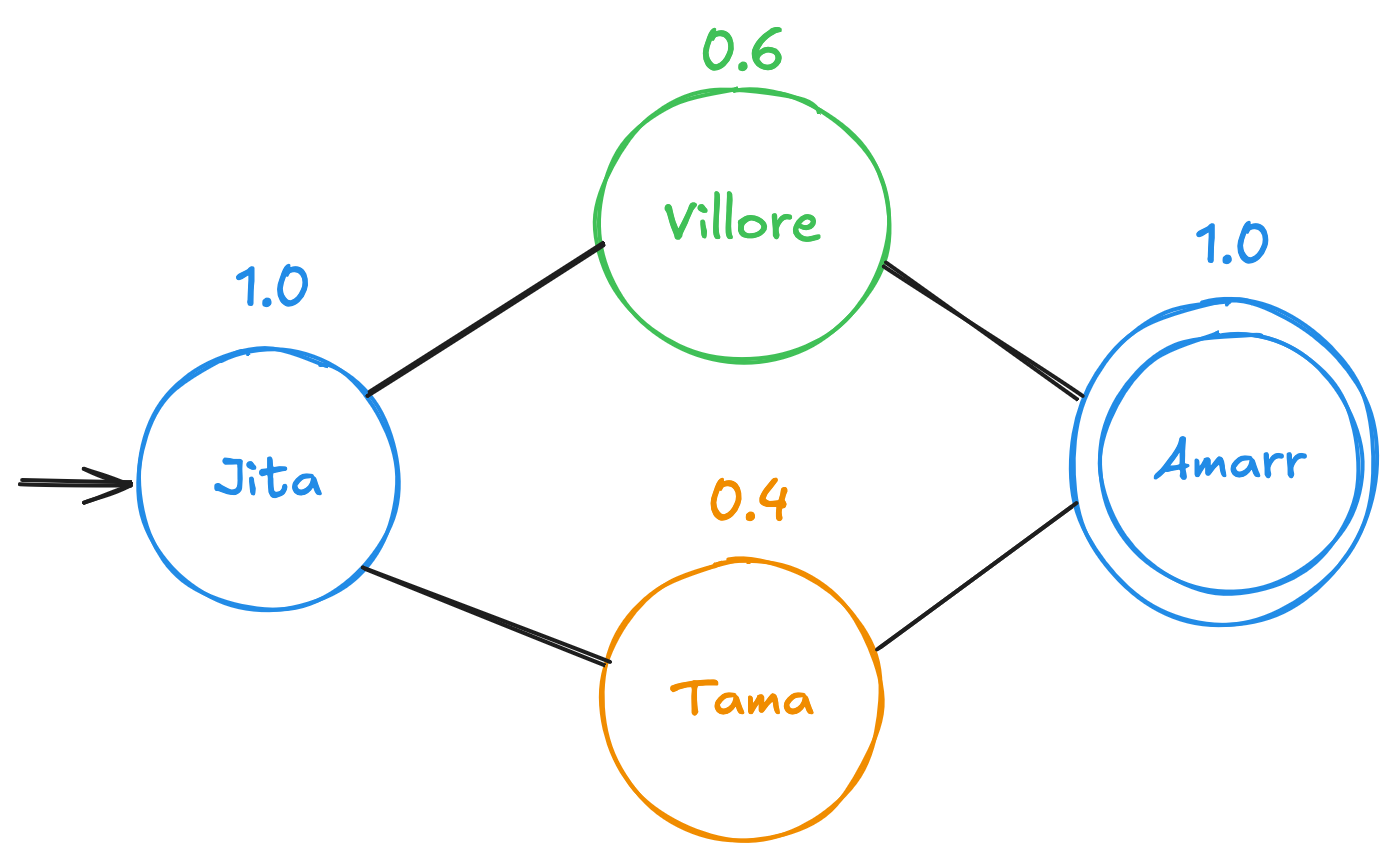
\includegraphics[width=0.5\linewidth]{images/useCase.png}
    \caption{In this image, three possible paths are considered.}
    \label{fig:useCase}
\end{figure}

In the previous figure, altough the safest route is $Villore \rightarrow Dodixie$, it is not the shortest. And assuming that every HS system is equally important (from a security status point of view), it is necessary to consider another function (heuristics are discussed in subsection \ref{sec:heuristics}).

\subsection{Heuristics}\label{sec:heuristics}

$A^*$ is a best-first algorithm. This means that after expanding a node, it will take the most promising next node. Then, it is possible to define a function $f(n)$ such as:
$$f(n) = g(n) + h(n)$$
\begin{itemize}
    \item $g(n)$ is the \textbf{cost function} or accumulated cost function from origin to the current node. In this case, it is possible to calculate it using the Dijkstra algorithm.
    \item $h(n)$ is the heuristic function calculated for each node. 
\end{itemize}

\subsubsection{The $h(n)$ function}

This fuction is calculated taking into account two possible parameters:

\begin{itemize}
    \item The distance from the current node $N$ to the destination $D$.
    \item The security status of the current system.
\end{itemize}

The system status plays an important role: depending on the value, a penalty factor may be applied in order to increase the cost $C_N$. For arbitrary reasons, the penalty in considered as $P = 10000$. 

The shortest path $r$ from current node $N$ to the destination $D$ is also considered - and calculated - using Dijkstra algorithm.

Therefore:

\[
h(n) =
\begin{cases}
(1 - \text{sec\_status) } + \text{r} , & \text{if  sec\_status} \geq 0.5 \\
|(1 - \text{sec\_status }) + (\text{r} \cdot \text{P})|, & \text{otherwise}
\end{cases}
\]

\bibliographystyle{johd}
\bibliography{bib}

\section*{Supplementary Files (optional)}
Any supplementary/additional files that should link to the main publication must be listed, with a corresponding number, title and option description. Supplementary files should also be cited in the main text.
Note: supplementary files will not be typeset so they must be provided in their final form. They will be assigned a DOI and linked to from the publication.

\end{document}